\section{Центрированные оптические системы. Тонкая линза. Фокусы и главные плоскости оптической системы. Оптические инструменты: лупа, телескоп и микроскоп.}
\subsection*{Центрированной оптической системой}
называют совокупность преломляющих и отражающих сред, отделённых друг от друга симметричными поверхностями, центры кривизны которых находятся на одной прямой. Эту прямую называют главной оптической осью системы.
\subsection*{Тонкая линза}
Линза --- прозрачное тело, изготовленное из оптически однородного материала, ограниченное двумя полированными выпуклыми или вогнутыми поверхностями.\\
Точки $O$ и $O'$ пересечения поверхностей линзы с главной оптической осью называются вершинами линзы. Расстоянием $d$ между вершинами называется толщина линзы. Линза считается тонкой, если $d << R_1$, $d << R_2$.\\
Формула тонкой линзы:
$$\frac{1}{F} = (n - 1) (\frac{1}{R_1} - \frac{1}{R_2})$$
\subsection{Фокусы и главные плоскости оптической системы.}
Если оптическая система превращает параллельный пучок света в сходящийся, то точка, в которой пересекаются лучи после прохождения системы называется фокусом. Две сопряжённые плоскости, отображающиеся с линейным увеличением $\beta =  \pm 1$, называются главными .
\subsection{Лупа}
Лупа --- это оптическая система, состоящая из одной или нескольких линз и предназначенная для наблюдения мелких предметов, расположенных на конечном расстоянии.\\
Если с расстояния $l_0$ смотреть на изображение, то $\Gamma = \frac{l_0}{F}$, где $F$ --- фокусное расстояние лупы. (Выведешь сам)
\subsection{Телескоп}
Телескоп --- система, включающая в себя объектив и окуляр. Причём передний фокус окуляра совмещён с задним фокусом объектива. При таком расположении элементов параллельный пучок, попадающий в объектив преобразуется в параллельный пучок на выходе из окуляра.\\
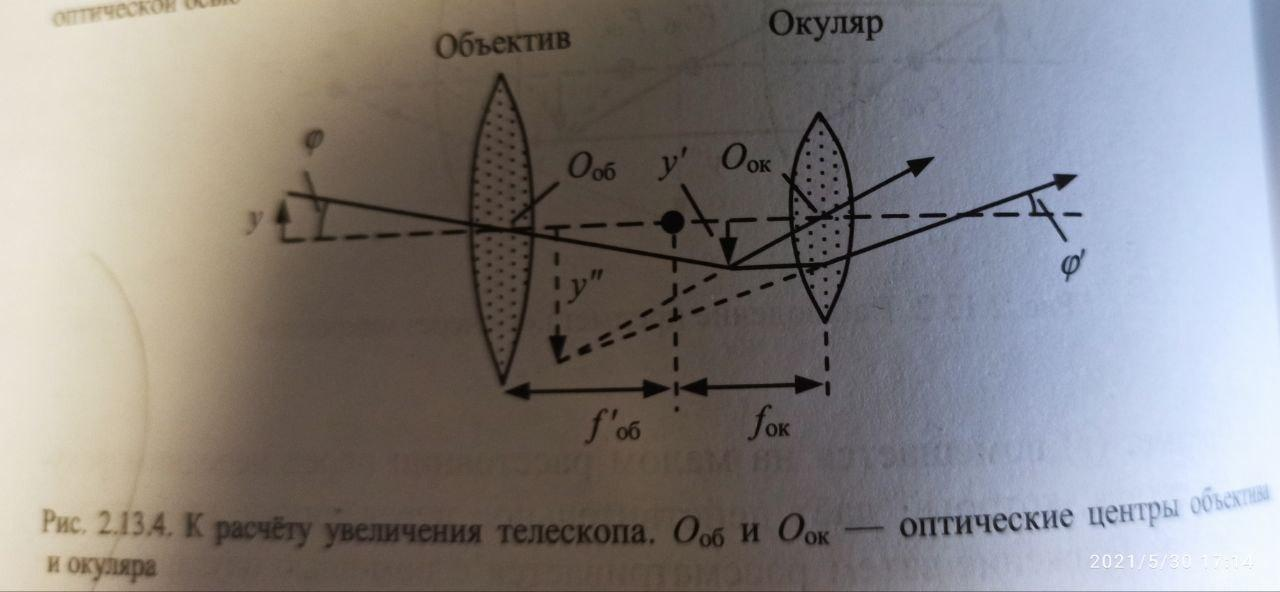
\includegraphics[width=\textwidth]{parts/img/p2_telescope.jpg}\\
$$\Gamma = \frac{F_{об}}{F_{ок}}$$

Фокусное расстояние окуляра как правило мало по сравнению с фокусным расстоянием объектива, что обеспечивает большое увеличение

\subsection{Микроскоп}
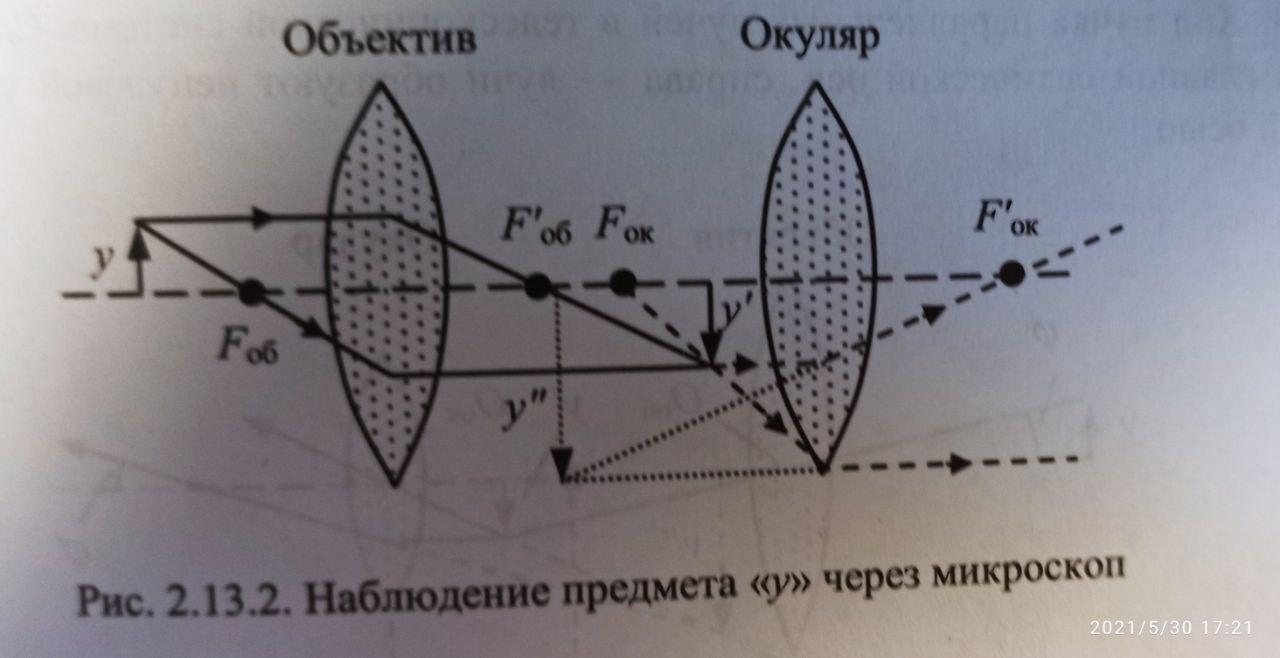
\includegraphics[width=\textwidth]{parts/img/p2_microscope.jpg} \\
Предмет (y) помещается на малом расстоянии перед передним фокусом объектива, который даёт действительное перевёрнутое изображение (y'). Это изображение затем рассматривается с помощью окуляра, действующего так же, как лупа.\\
Увеличение окуляра связано с тем, что конечное изображение (y'') видно под большим углом, чем при непосредственном наблюдении глазом.